\begin{center} 
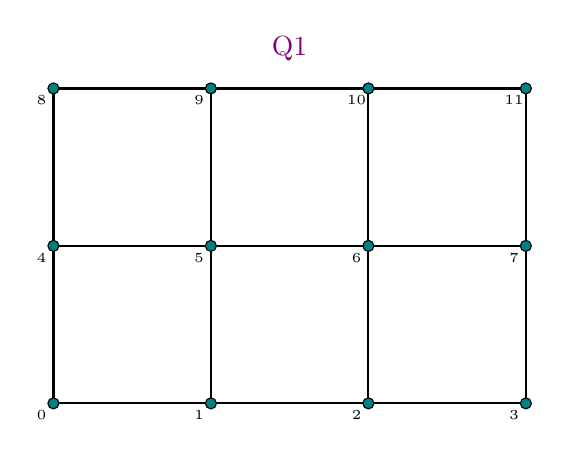
\begin{tikzpicture} 
\node[violet] at (3,4.5) {Q1}; 
\draw[thick] (0,0) -- (6,0) -- (6,4) -- (0,4) -- cycle; 
\draw[thick] (0,2) -- (6,2) ; 
\draw[thick] (2,0) -- (2,4) ; 
\draw[thick] (4,0) -- (4,4) ; 
\draw[black,fill=teal] ( 0.000000 , 0.000000)     circle (2pt); 
\node[] at ( -0.150000, -0.150000 ) {\tiny 0 }; 
\draw[black,fill=teal] ( 2.000000 , 0.000000)     circle (2pt); 
\node[] at ( 1.850000, -0.150000 ) {\tiny 1 }; 
\draw[black,fill=teal] ( 4.000000 , 0.000000)     circle (2pt); 
\node[] at ( 3.850000, -0.150000 ) {\tiny 2 }; 
\draw[black,fill=teal] ( 6.000000 , 0.000000)     circle (2pt); 
\node[] at ( 5.850000, -0.150000 ) {\tiny 3 }; 
\draw[black,fill=teal] ( 0.000000 , 2.000000)     circle (2pt); 
\node[] at ( -0.150000, 1.850000 ) {\tiny 4 }; 
\draw[black,fill=teal] ( 2.000000 , 2.000000)     circle (2pt); 
\node[] at ( 1.850000, 1.850000 ) {\tiny 5 }; 
\draw[black,fill=teal] ( 4.000000 , 2.000000)     circle (2pt); 
\node[] at ( 3.850000, 1.850000 ) {\tiny 6 }; 
\draw[black,fill=teal] ( 6.000000 , 2.000000)     circle (2pt); 
\node[] at ( 5.850000, 1.850000 ) {\tiny 7 }; 
\draw[black,fill=teal] ( 0.000000 , 4.000000)     circle (2pt); 
\node[] at ( -0.150000, 3.850000 ) {\tiny 8 }; 
\draw[black,fill=teal] ( 2.000000 , 4.000000)     circle (2pt); 
\node[] at ( 1.850000, 3.850000 ) {\tiny 9 }; 
\draw[black,fill=teal] ( 4.000000 , 4.000000)     circle (2pt); 
\node[] at ( 3.850000, 3.850000 ) {\tiny 10 }; 
\draw[black,fill=teal] ( 6.000000 , 4.000000)     circle (2pt); 
\node[] at ( 5.850000, 3.850000 ) {\tiny 11 }; 
\end{tikzpicture} 
\end{center} 
